% mainfile: ../../../../master.tex
\subsection{Extraction of total DNA and RNA from marine sample}
% The part of the label after the colon must match the file name. Otherwise,
% conditional compilation based on task labels does NOT work.
\label{task:20180109_cj0}
\tags{dna,rna,lab,extr}
\authors{cj}
%\files{}
%\persons{}

\subsubsection{Introduction}

This protocol was adapted from \citet{schneider2017extraction} and \citet{chomczynski2006single} to simultaneously extract DNA and RNA from marine samples.

The previous extraction I performed following this protocol failed (cf. section \ref{task:20180103_cj0}) so I want to repeat this experiment to extract the RNA and DNA from Mia's culture (she suspect that this one contains cyanobacteria) \texttt{20170623 SB5 0m F/2}.


\subsubsection{Lysis and homogenisation}

\begin{enumerate}
\item 2 mL of cultures split in 2 2mL-Eppendorf tubes.
\item Centrifuge at 9300 RCF (10000 rpm) at 4\degree C for 5 min (Eppendorf 5415R).
\comment{I can see a light green pellet.} 
\item Remove the supernatent.
\item Add 2 mL of denaturing solution.
\item Vortex.
\item Incubate at room temperature for 10 min.
\comment{The original procedure suggest I repeat the extraction with an extra 2mL of denaturing solution. I did not repeat this step to reduce the volume I will be working with.}
\item Transfer the lysate into a fresh 15 mL Falcon tube.
\end{enumerate}


\subsubsection{Simultaneous DNA and RNA extraction}
\begin{enumerate}
\item Add 0.1 volume of 2~M sodium acetate pH 4.
\mistake{I added too much, it was supposed to be 0.1 vol so I should not have added 0.4mL of sodium acetate buffer to each tube, but 60 \uL in each eppendorf tube.}
\item Add 1 volume of phenol pH 4.
\item Mix thoroughly by inversion.
\item Add 0.2 volume of chloroform:isoamyl alcohol (24:1).
\item Cool on ice for 15 min.
\comment{I believe it remained on ice for longer than 15 min}
\item Centrifuge for 20 min at 7200 g at 4\degree C (during the centrifugation, the mixture should separate into a lower phenol phase and interphase and an upper aqueous phase).
\comment{After centrifugation, I am unable to see the two phases, so I combined all the contents of the 6 eppendorf tubes into one 15 mL falcon tube, and I added 1mL of chloroform isoamyl alcohol and I repeat the centrifugation step with a different rotor so at 5000 RPM.}
\item Transfer carefully the supernatent (aqueous phase) which contains mostly RNA to a clean Falcon tube.
\comment{Here I am able to transfer easely 3 mL of supernatent.}
\item Add 2~mL of 2~M sodium acetate buffer pH 4.
\item Mix thoroughly by inversion.
\item Centrifuge for 20 min at 4\degree C.
\item Transfer carefully the upper phase to the already collected aqueous phase.
\item For later DNA isolation, add 1 volume of Tris-base pH 10.5 to the phenolic phase and mix well.
\comment{Here I transfered the phenol phase from the 15 mL Falcon tube to a fresh 50 mL Falcon tube so I am sure I will be able to add enough alkaline solution to bring the pH back to neutral.}
\comment{To avoid the same issue as last time, I check the pH with pH paper to ensure the pH is back to neutral/alkaline.}
\item Continue with RNA precipitation. 
\end{enumerate}

\subsubsection{RNA isolation}
\begin{enumerate}
\item Add 1 volume of chloroform:isoamyl alcohol (24:1).
\item Incubate at -20\degree C for at least 15 min (but no longer than 1h).
\item Centrifuge again for 20 min at 4\degree C to separate the two phases.
\item Transfer the aqueous upper plase to a fresh tube.
\item Repeat the chloroform extraction by adding 2~mL of 2~M sodium acetate buffer to the organic phase, mix and centrifuge again, and finally transfer the supernatent to the already collected aqueous phase.
\item Add 1/500 volume of glycogen (20 mg/mL) \sidenote{The glycogen solution was prepared by Stephen back in 2014 and kept at -20\degree C.}
\item Mix vigorously.
\item Add 1 volume of isopropanol to precipitate RNA.
\item Incubate samples at -20\degree C overnight. 
\comment{By incubating overnight it will precipitate everything so it is very likely that I will also precipitate some contaminants. But at least I am sure all the RNA will be precipitated and I can just perform more washing steps afterwards.}
\item Continue with DNA isolation.
\end{enumerate}

\subsubsection{DNA isolation}
\begin{enumerate}
\item Mix tube containing the extracted DNA obtained from previous steps.
\item Centrifuge again for 20 min at 5000 RPM at 4\degree C to separate the two phases.
\item Transfer the upper aqueous phase into fresh tubes (at this point, check pH again with pH paper).
\item Add 2~mL of 1~M Tris-base pH 10.5 to the lower phenolic phase and repeat mixing and centrifugation to separate the two phases.
\item Transfer the upper aqueous phase to the already collected aqueous phase (at this point, check pH again with pH paper).
\item Add 1 volume of chloroform:isoamyl alcohol (24:1) to the aqueous phase.
\item Mix thoroughly by inversion.
\item Centrifuge for 10 min at 4\degree C to separate the two phases/
\mistake{The 50 mL tube containing my DNA broke during the centrifugation ... I thought the adaptor I place in the swinging bucket was for 50 mL Falcon tubes, but apparently it was not. That's the only reason I can think of for the tube to break in the centrifuge.}
\end{enumerate}

The tube that broke in the centrifuge contained chloroform as shown in figure \ref{fig:20180110_broken_tube}. For safety reason, I stop my experiment at this stage: I close the fumehood and I will wait until tomorrow to clean up to make sure most of the chloroform is evaporated. 

I will have the start again this experiment.

\begin{figure}[H] % position of the figure 
    \centering
    \caption{Picture of the broken tube.}
    \label{fig:20180110_broken_tube}
    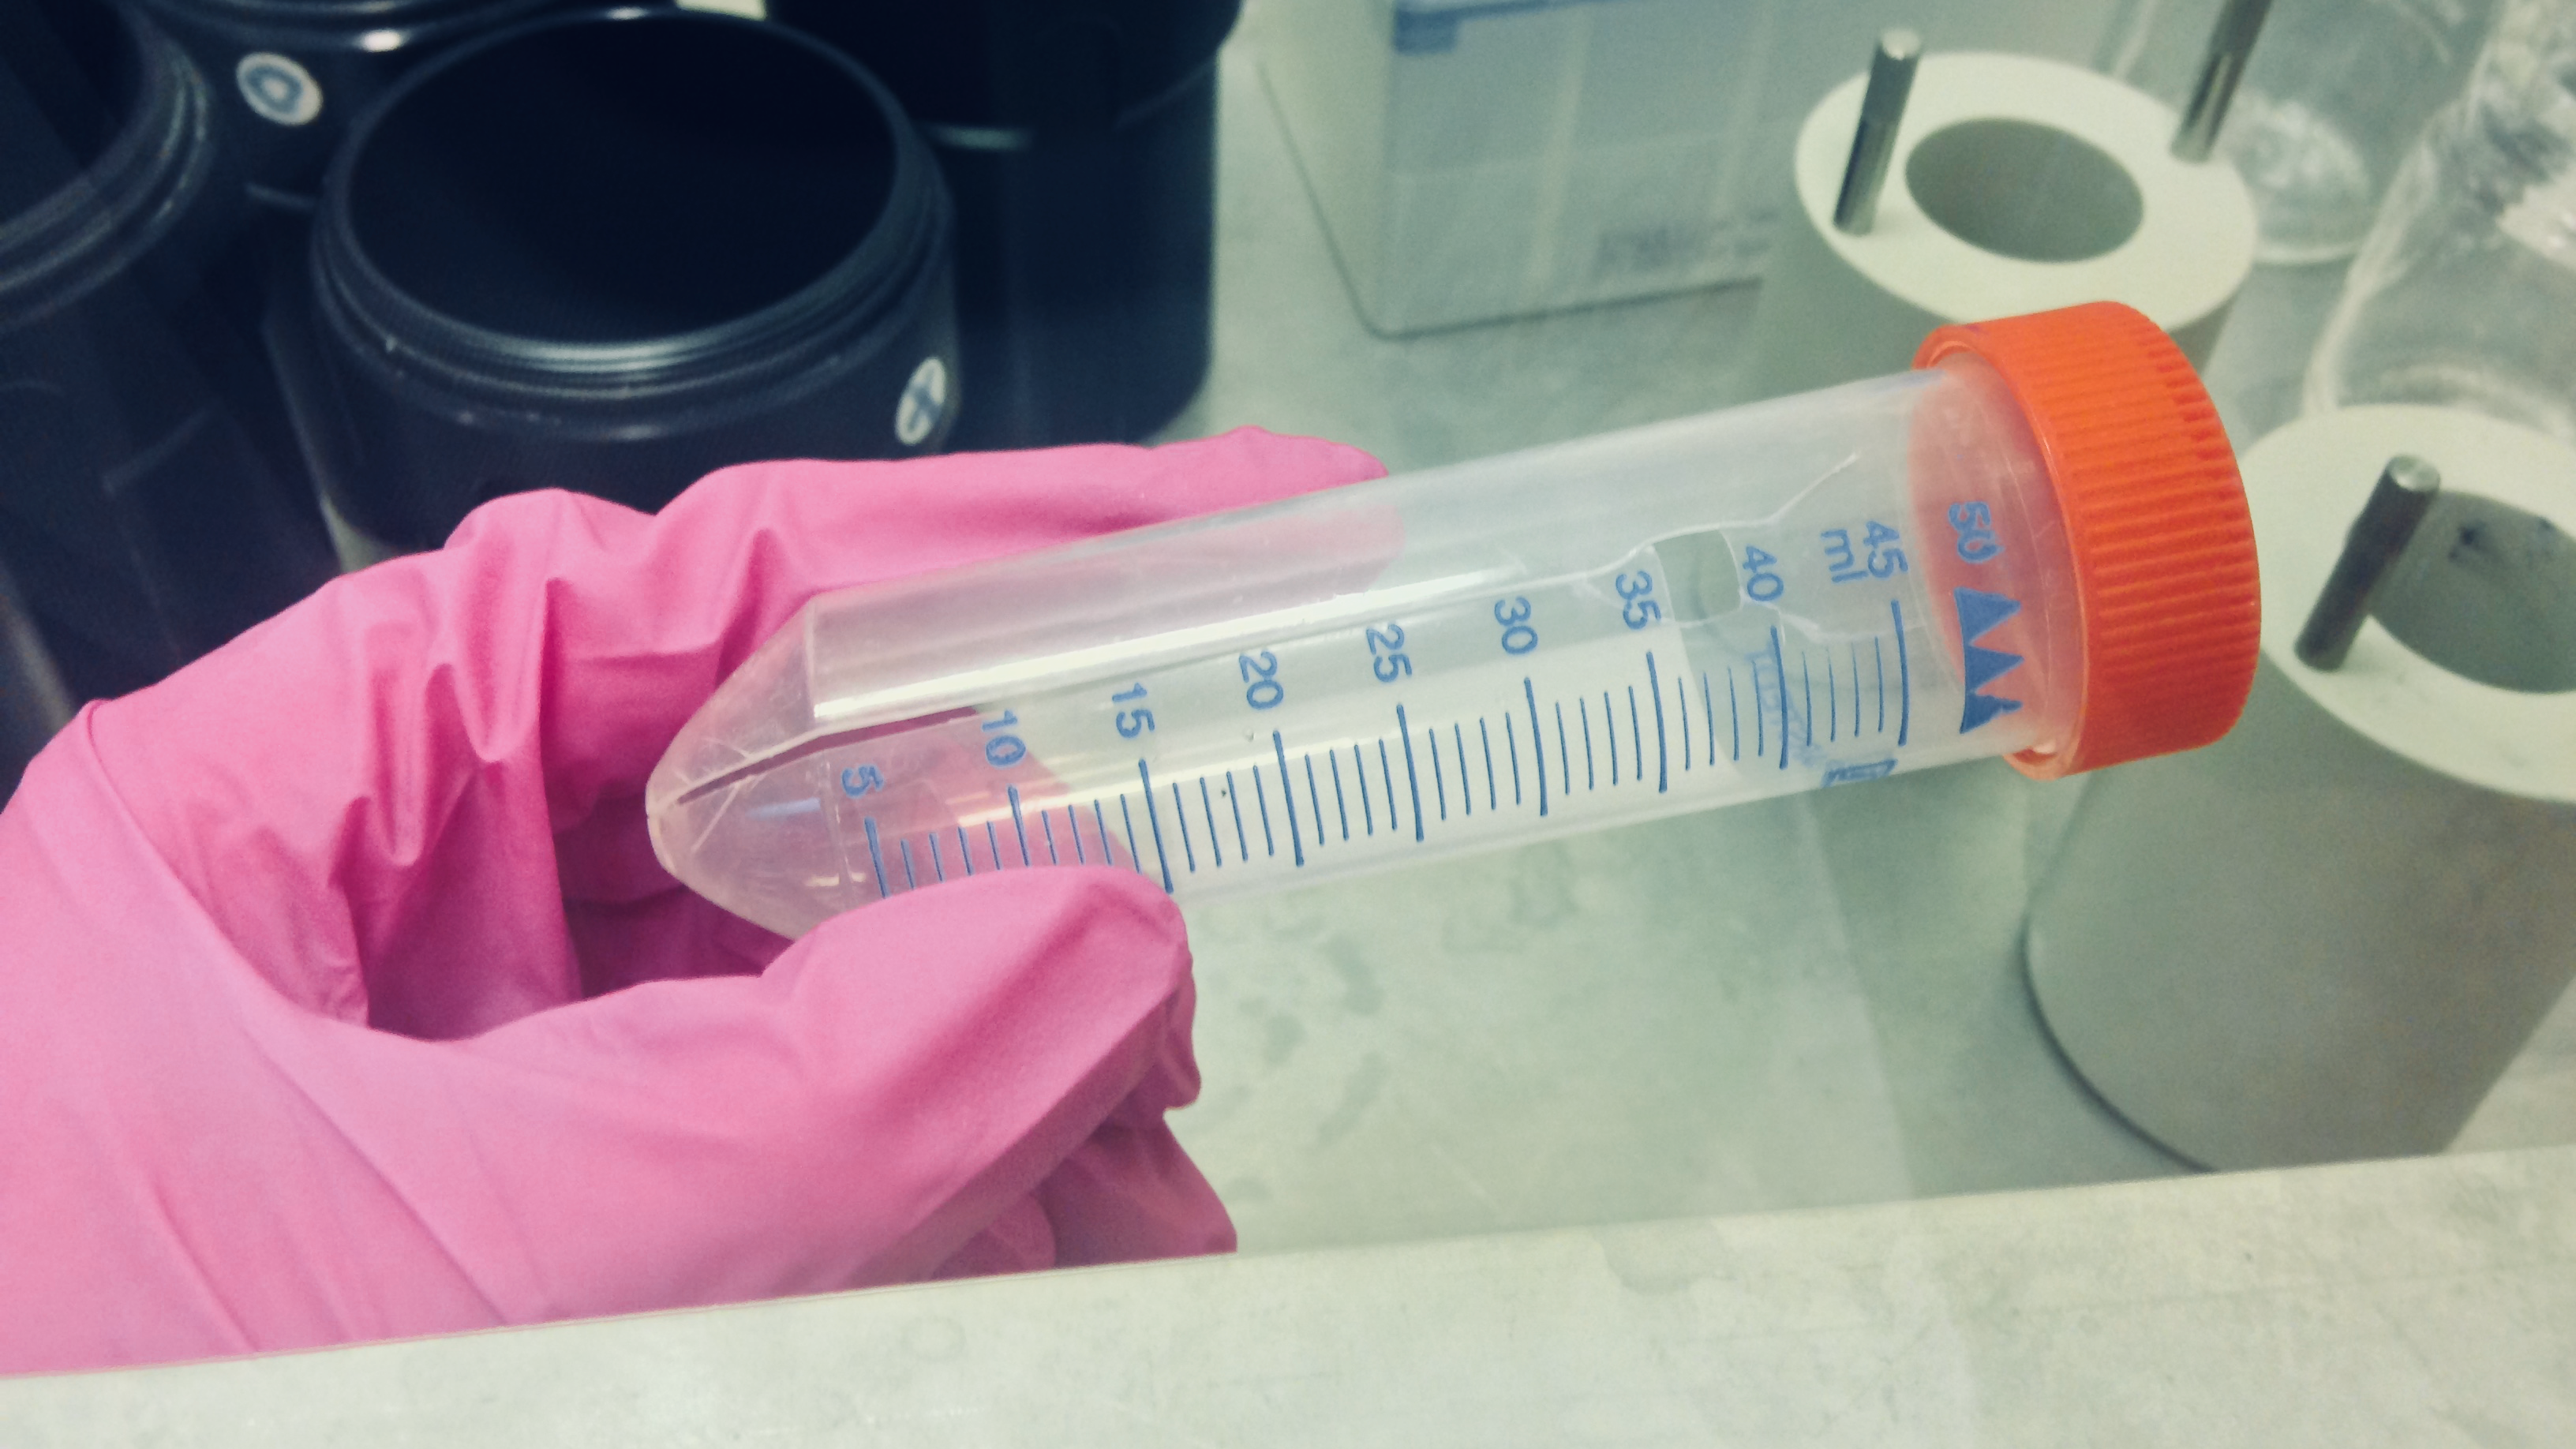
\includegraphics[width=\textwidth]{graphics/pic/20180110_broken_tube.png}
\end{figure}

